\documentclass[output=paper]{langsci/langscibook} 
\author{Isabelle Udry\orcid{}\affiliation{University of Fribourg, Institut de Plurilinguisme; Zurich University of Teacher Education} and Jan Vanhove\orcid{}\affiliation{University of Fribourg, Institut de Plurilinguisme}}
\title[The stability of language aptitude]
      {The stability of language aptitude: Insights from a longitudinal study on young learners’ language analytic abilities}
\abstract{An enduring question in aptitude research is the extent to which aptitude is a stable trait or a time-varying attribute. If aptitude were a perfectly stable trait, interindividual differences in aptitude at one point in time should be perfectly correlated with interindividual differences at a later point in time. However, raw test scores are affected by measurement error, a result of which is that correlations between raw test scores at different points in time underestimate the correlations between the actual skills measured by these tests at different points in time. The analyses of the longitudinal LAPS~II aptitude data ($n=636$; translated and adapted versions of MLAT and PLAB subtests) take into account measurement error and indicate that the children’s ability to solve the MLAT and PLAB tests at the first data collection (autumn 2017, mean age: 10;5 years) and their ability at the third data collection (spring 2019, mean age: 12;1 years) are correlated at $\rho = 0.74$ (95\% CrI: [0.69, 0.79]). This suggests that the ability to solve the two aptitude tests is not a perfectly stable interindividual trait, but that, by and large, interindividual differences are nonetheless maintained over the course of one-and-a-half years of cognitive development.}
\IfFileExists{../localcommands.tex}{
  \addbibresource{localbibliography.bib}
  % add all extra packages you need to load to this file

\usepackage{tabularx,multicol}
\usepackage{url}
\urlstyle{same}

\usepackage{listings}
\lstset{basicstyle=\ttfamily,tabsize=2,breaklines=true}

%\usepackage{langsci-optional}
\usepackage{langsci-lgr}
\usepackage{langsci-gb4e}
\usepackage{langsci-optional}

\usepackage{enumitem}
\usepackage[group-digits=false, detect-weight=true]{siunitx}

\usepackage{todonotes}

  \newcommand*{\orcid}{}
 
  %% hyphenation points for line breaks
%% Normally, automatic hyphenation in LaTeX is very good
%% If a word is mis-hyphenated, add it to this file
%%
%% add information to TeX file before \begin{document} with:
%% %% hyphenation points for line breaks
%% Normally, automatic hyphenation in LaTeX is very good
%% If a word is mis-hyphenated, add it to this file
%%
%% add information to TeX file before \begin{document} with:
%% %% hyphenation points for line breaks
%% Normally, automatic hyphenation in LaTeX is very good
%% If a word is mis-hyphenated, add it to this file
%%
%% add information to TeX file before \begin{document} with:
%% \include{localhyphenation}
\hyphenation{
affri-ca-te
affri-ca-tes 
Soa-res
scru-ti-ny
me-ta-cog-ni-tion
}

\hyphenation{
affri-ca-te
affri-ca-tes 
Soa-res
scru-ti-ny
me-ta-cog-ni-tion
}

\hyphenation{
affri-ca-te
affri-ca-tes 
Soa-res
scru-ti-ny
me-ta-cog-ni-tion
}
 
  \togglepaper[1]%%chapternumber
}{}

\begin{document}
\maketitle 

\section{Introduction}

Language aptitude as defined by \citet{Carroll1958} consists of four basic components, i.e. phonetic coding ability, grammatical sensitivity, inductive ability, and rote memory (see Chapter 1 for a discussion). One of the key debates in aptitude research is whether the construct is a stable characteristic or an ability that can be developed. Addressing this issue contributes to establishing a conceptual aptitude framework and can clarify the question if language learning may be enhanced by specific aptitude treatments. Despite educational and theoretical relevance, studies dealing with the stability of language aptitude in general, and particularly in children, remain scarce. 

Aptitude stability can be explored in the data in different ways: 1. Researchers consider average aptitude test scores achieved by one or several groups of participants (we refer to this as the \textit{group averages} approach) or 2. they determine an individual’s relative ranking within the group (which we call the \textit{relative ranking} approach). In both approaches, researchers then look for patterns, either cross-sectionally by comparing groups at different developmental stages or longitudinally by comparing data obtained at different times from the same individuals or groups. How these patterns are explained depends amongst other things on the researchers’ conceptualization of construct stability: Developmental changes (expressed as age-related gain scores obtained in an aptitude test) can be interpreted as construct malleability. Alternatively, such changes can be seen as indicating construct stability if an individual’s ranking within the population or group remains largely constant, despite increased aptitude scores at different times of testing. 

In our view, describing changes in average scores only is scarcely insightful in our context, as children are expected to score higher on aptitude tests as they mature, namely due to developmental changes in cognition. It would be more revealing to find out if they progress at the same rate (indicating a general developmental pattern and a stable trait) or differentially (indicating individual developmental patterns and therefore a malleable ability). Depending on whether the \textit{group averages} and \textit{relative ranking} change, different conclusions may be drawn: 

\begin{enumerate}
\item Group averages and the relative ranking both change: possible indication of malleability
\item Group averages change, the relative ranking remains the same: possible indication of stability
\item Group averages do not change, but the relative ranking does (due to some individuals progressing while others’ ability to solve the test decreases): possible indication of malleability
\item Neither group averages nor relative rankings change: possible indication of stability
\end{enumerate}

Several authors assume that language aptitude is subject to change (see for instance \citealt{GrigorenkoEtAl2000}, \citealt{Singleton2017}). Their view runs contrary to earlier conceptions, as expressed by \citet[86]{Carroll1981} who described language aptitude as “relatively hard to modify in any significant way.” In the same article, the author (1981: 84) slightly qualified his statement by adding that the initial aptitude components could be modelled as “more or less enduring characteristics” and as a “current state”.  

The view of a stable characteristic has been substantiated in particular with evidence from a long-term study by \citet{Skehan1986} and \citet{SkehanDucroquet1988} which found that some measures of L1 development, namely L1 vocabulary and mean length of utterance,  were predictive of L2 aptitude measures assessed 13 years later in the same participants.

It is worth remembering that Carroll, who first conceptualized language aptitude, was mainly concerned with capturing a snapshot of people’s potential before they started learning a language in order to predict their later L2 achievement. Whether this potential was innate or malleable was not an explicit question in these early stages of aptitude research. However, as early as 1964, careful readers could detect Carroll’s awareness of the issue tucked away in a footnote, stating that the extent to which “the behaviour measured on the aptitude tests … can be modified by training” would still “need to be investigated” \citep[89]{Carroll1964}. Later, he expressed doubts about the feasibility of such a training, stating that “there are some general grounds for pessimism regarding the teaching of aptitudinal skills” (1973: 8), contributing to his view was the fact that not enough research had been conducted on the matter. 

\section{Review of the literature} 

Studies investigating the stability of language aptitude are rather scarce and usually underpinned by the hypothesis that aptitude is shaped by language experience. \citet{RoehrBrackinTellier2019} examined the relationship and development of language aptitude and metalinguistic awareness with 111 anglophone beginning learners of L2 French aged 8 to 9 years. In phase 1 (16 weeks) of the project participants were divided into four groups that were taught either German, Italian, Esperanto, or Esperanto with an added focus-on-form element. In phase 2 (16 weeks), all children learnt French with an element of focus-on-form. The authors administered tests for aptitude (an adaptation of the MLAT-E by \citet{CarrollSapon1976} for British English speakers), metalinguistic awareness, and L2 French proficiency (listening, reading, writing, grammar) in a pretest--posttest design which included immediate and delayed posttests for L2 French. The authors detected increases in aptitude test scores with a medium effect size. According to the “\textit{group averages}” definition of stability given in the introduction, they concluded that language aptitude was dynamic in the sample. Moreover, the authors found that children who performed well on the aptitude pretest also did well on the aptitude posttest, and vice versa, suggesting a largely stable ranking. This finding was interpreted in favour of the aptitude test’s predictive value for young learners’ L2 performance. However, based on the “\textit{relative ranking}” definition of stability, we argue that this finding could also point to the stability of language aptitude.

An increase in aptitude test scores with age was also detected by \citet{SuarezVilagran2010} who administered Spanish and Catalan translations of the MLAT-E (see \sectref{sec:01:2.2}) to 629 Spanish-Catalan bilingual learners of English aged 8 to 15. She observed a considerable increase in aptitude scores between ages 8 and 9. After the age of ten, gain scores weren’t as large, and the author therefore suggests that aptitude may stabilize around age 11.

\citet{KissNikolov2005} tested aptitude (with a Hungarian MLAT based test), motivation, and English proficiency (listening, reading, writing) in 419 12-year-old L2 English learners. The authors also recorded time of exposure to English at school and in private tuition which ranged considerably from 100 to 1085 hours ($M= 343; \text{SD}= 131$). Kiss and Nikolov explored the effects of language experience on aptitude by establishing correlations between time spent on learning and aptitude test scores. This correlation being weak, they concluded that language aptitude in the Carrollian sense did not improve with “the amount of time used for practice and exposure” (\citealt{KissNikolov2005}: 134).

In a subsequent study, \citet{Kiss2009} reconsidered the interplay between language experience and aptitude. The author administered a Hungarian aptitude test for young learners to 52 Hungarian children. The aim was to select 26 8-year-olds for a newly established bilingual English-Hungarian teaching program. The author compared the results from all 8-year-old children to those from 12-year-olds from a previous study. She found that the 12-year-olds performed better on the vocabulary learning subtest than their younger counterparts. Kiss (2009: 268f) speculates that these differences are owed to the older children’s greater language learning experience and better developed strategies. Based on the idea that aptitude malleability is evidenced by increased group averages, the author concluded that language aptitude is dynamic, at least up to the age of 12. 

A frequently cited study by \citet{SafarKormos2008} addressed the stability of the construct with 61 Hungarian learners of English aged 15 to 16 years. The authors assessed language aptitude and short-term memory at the beginning and end of the academic year. 41 participants followed an English-Hungarian bilingual program (with sixteen 45 min English lessons per week\,+\,4\,×\,45 min. CLIL per week) and 21 participants were from a regular Hungarian secondary school (with 4\,×\,45 English lessons a week predominantly communicative with some focus-on-form instruction). Aptitude test scores increased significantly in both groups between the two data collections, independent of the intensity of instruction. Learners in the bilingual program, however, improved more than their counterparts in the regular setting. Based on these findings, the authors concluded that language aptitude is dynamic and changes with language experience. The authors also stated that language aptitude appears to be less relevant in communicative teaching with a focus-on-form element. It seems worth noting that some information on other potential influences, such as general learning abilities or admission criteria for the bilingual program, may have contributed to explaining the results. 

In summary, current empirical findings suggest that language aptitude is dynamic in children younger than 12. Primary school children score higher on aptitude tests as they get older, with important increases in test scores being observed between 8 and 9 years (\citealt{MiltonAlexiou2006}, \citealt{Kiss2009}, \citealt{SuarezMunoz2011}). These findings are based on the \textit{group averages} definition of stability, i.e. a gradual improvement in the average performance of groups of children. 

\section{Method}

We investigated the stability of language aptitude in primary school children over a period of 1.5 years. To this aim, we defined language aptitude as language analysis \citep{Skehan1998}, i.e. the grammatical sensitivity and inductive ability components from \citegen{Carroll1958} construct definition (see also Chapter 1 for a discussion). As outlined earlier, primary school children are still maturing cognitively, and their aptitude scores are expected to improve with age. Therefore, we were more interested in the extent to which individual differences in language aptitude remain stable over time, i.e. whether participants who perform well relative to other participants on an aptitude test at one point T1 will still do so at a later time of testing T2 (or even T3, as in our data). This can be inferred from the correlation between the participants’ test results at T1 and T2 (and T3): The stronger this correlation is, the more stable interindividual differences in language aptitude are. 

 \section{Participants and procedure}


The study design is fully described in Chapter 2 and will be summarised briefly: To assess language analytic ability (i.e. grammatical sensitivity and inductive ability), we adapted the following tests for German-speaking young learners\footnote{We would like to thank Charles W. Stansfield for permission to translate and adapt parts of the MLAT-E and PLAB for this study.}: MLAT-E subpart “Matching Words” on grammatical sensitivity (\citealt{CarrollSapon1976}) and PLAB subpart 4 on inductive ability \citep{PimsleurEtAl2004}. The same participants from LAPS II (4\textsuperscript{th} and 5\textsuperscript{th} graders at T1), completed these tests at three different times T1--T3: T1 = Autumn 2017 (mean age 10;5); T2 = Spring 2018 (mean age 11); T3 = Spring 2019 (mean age 12;1). A total of 636 participants completed the tests between T1 and T3. Figures 10.1 and 10.2 show the correlations between the test scores from T1 to T3. \tabref{tab:10:1} summarizes the test results. 

   
\begin{figure}
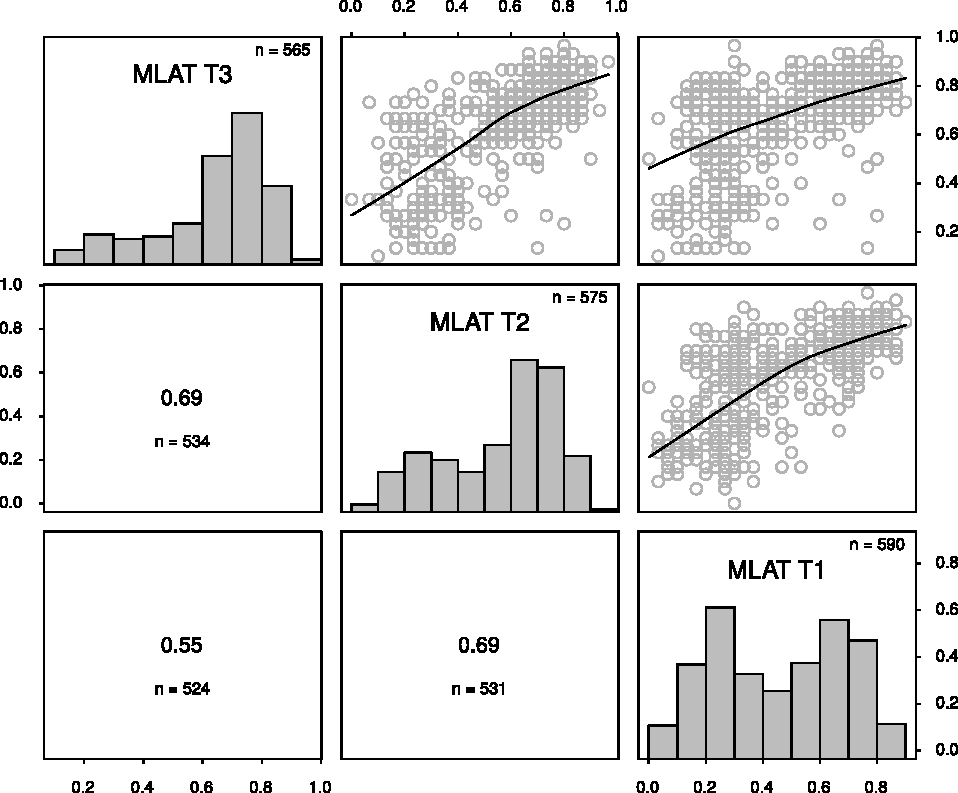
\includegraphics[width=\textwidth]{figures/figure10.1.pdf}
\caption{\label{fig:10:1} Scatterplot matrices with the MLAT results at the three data collections. Upper triangle: Scatterplots with scatterplot smoothers. Main diagonal: Histograms. Lower triangle: Pearson correlation coefficients as well as the number of data points on which these were based.}
\end{figure}

  
\begin{figure}
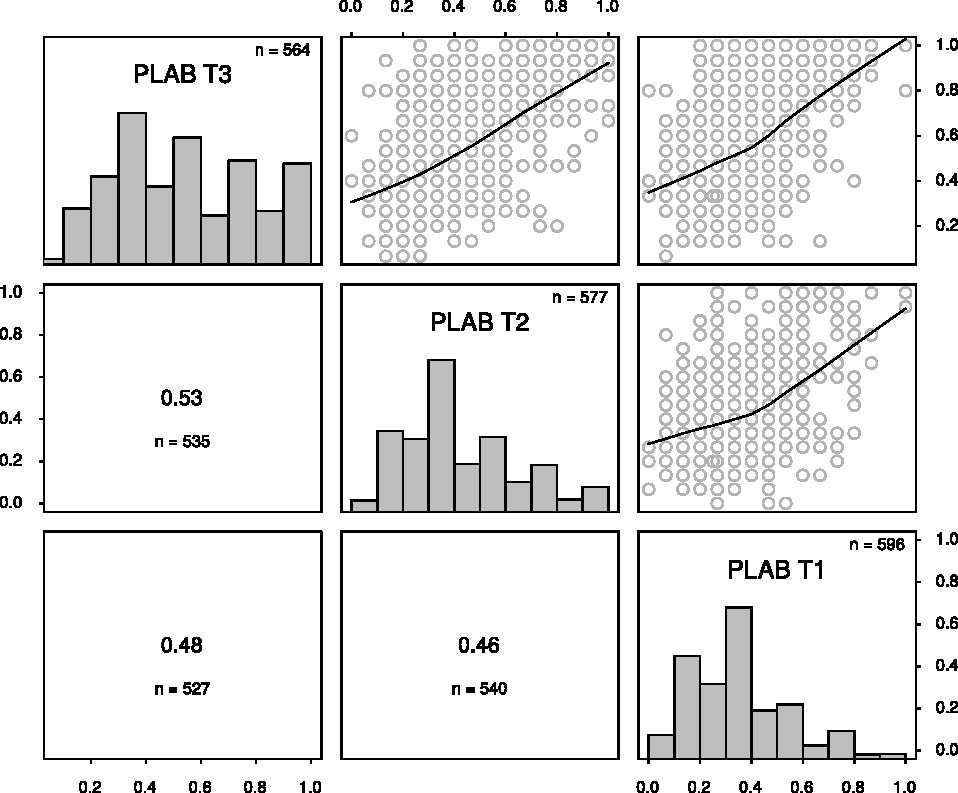
\includegraphics[width=\textwidth]{figures/figure10.2.pdf}
\caption{\label{fig:10:2}PLAB results and correlations at different times of testing T1--T3. Scatterplot matrices with the MLAT results at the three data collections. Upper triangle: Scatterplots with scatterplot smoothers. Main diagonal: Histograms. Lower triangle: Pearson correlation coefficients as well as the number of data points on which these were based.}
\end{figure}

\begin{table}
\caption{\label{tab:10:1}MLAT and PLAB test results at T1--T3. The total number of participants completing the tests at different times between T1--T3 is 636. MLAT has 30 items and PLAB 15.}
\begin{tabular}{ll ccc}
\lsptoprule
{Test} & {Time} & {Participants} & {Mean\footnote{Proportion of correct answers}} & {SD}\\\midrule
{MLAT} & {T1} & {590} & {0.48} & {0.23}\\
       & {T2} & {575} & {0.58} & {0.22}\\
       & {T3} & {565} & {0.66} & {0.19}\\
{PLAB} & {T1} & {596} & {0.37} & {0.19}\\
       & {T2} & {577} & {0.44} & {0.22}\\
       & {T3} & {564} & {0.56} & {0.25}\\
\lspbottomrule
\end{tabular}
\end{table}

Clearly, the results from the three testing times do not correlate perfectly (this would be indicated by a correlation coefficient of +1). Even if the ability to solve the MLAT or the PLAB were interindividually stable, we would still not expect to see a perfect correlation. This is due to measurement error: If two latent variables that correlate perfectly with each other are measured imperfectly, these measurements will still not yield a perfect correlation. 

If we knew the measurement error or the reliability coefficient of the tests, we could solve this problem by calculating disattenuated correlations. While we do not know the actual reliability of the instruments, we can estimate them. The reliability coefficients (\textit{ω\textsubscript{RT,}}, \citealt{McNeish2018}, \citealt{Revelle2019}) for the MLAT variable are 0.90 (T1), 0.89 (T2) and 0.88 (T3); for PLAB: 0.74 (T1), 0.80 (T2) and 0.84 (T3). If we use these values to disattenuate the correlations (using the correct.cor() function in the psych package for R, \citealt{Revelle2018}), we obtain the values in \tabref{tab:10:2}.



\begin{table}
\caption{\label{tab:10:2}\label{tab:10:3}Disattenuated correlations MLAT and PLAB}
\begin{tabular}{lcc cc}
\lsptoprule
     & \multicolumn{2}{c}{MLAT} & \multicolumn{2}{c}{PLAB}\\\cmidrule(lr){2-3}\cmidrule(lr){4-5}
     & {T1} & {T2}     & {T1} & {T2}\\\midrule
{T2} & {0.77} &        & {0.60} & \\
{T3} & {0.62} & {0.78} & {0.61} & {0.65}\\
\lspbottomrule
\end{tabular}
\end{table}


While computing disattenuated correlation coefficients is fairly straightforward, this analysis does not consider the dependence that exists between the tests: The MLAT scores for T1, T2 and T3 are based on the same test items, and the same goes for the PLAB scores. To take these dependencies into account, we ran an alternative, if more involved, analysis in which the participants’ item-level responses were modelled. This analysis was run using generalized (logistic) mixed-effects models, which are capable of estimating the participants’ latent abilities as well as the items’ latent difficulties.

In language research, analyses based on mixed-effects models usually focus on the fixed effects, but in our case, it is the random effects that are of particular interest. For each participant, the latent ability to solve the MLAT and PLAB can be estimated for T1, T2 and T3. Also, the correlations between the participants’ estimated latent abilities at T1, T2 and T3 can be estimated. In doing so, the analysis can also take into account the fact that items vary in their difficulty and that the relative difficulty of the test items may vary between T1, T2 and T3. 

We fitted three models: one on the MLAT responses, one on the PLAB responses and one on all responses combined. The models we fitted were Bayesian generalized (logistic) mixed-effects models; for our purposes, Bayesian models have the advantage that they can not only estimate the correlation between the participants’ latent abilities at T1, T2 and T3, but also quantify the uncertainty about this estimation. The models were fitted using the brm() function in the brms package for R \citep{Buerkner2017}. ``Result'' is a binary variable that indicates for each individual response whether it was correct (1) or not (0). ``Time'' is a categorical variable with three levels (T1, T2, T3), ``Item'' is a categorical variable specifying the test item, and ``StudentID'' is a categorical variable specifying the participant. The three models were specified as follows (in brms notation):

\begin{lstlisting}
m <- brm(result ~ 0 + Time + (0 + Time | Item) + (0 + Time | StudentID), data = d, family = bernoulli(link = "logit"), cores = 4, iter = 4000, warmup = 1000)
\end{lstlisting}

This model estimates (a) the probability (in logits) of a response being correct at Times 1, 2 and 3, (b) between-item differences in this probability, (c) between-participant differences in this probability, (d) the correlations among the between-item differences at Times 1, 2 and 3, and (e) the correlations among the between-participant difference at Times 1, 2 and 3. For our purposes, (e) is what is important, viz., the extent to which differences among the participants’ abilities at Time 1 are maintained at Times 2 and 3.

\section{Results}

The MLAT model was fitted on 51,875 responses (30 items\,×\,636 participants\,×\,3 data collections, with some missing data); the PLAB model was fitted on 26,044 responses (15 items\,×\,636 participants\,×\,3 data collections, with some missing data); the combined model was fitted on 77,919 responses (45 items\,×\,636 participants\,×\,3 data collections, with some missing data).

Tables~\ref{tab:10:4}--\ref{tab:10:6} summarise the main results pertinent to our research question. The full model output can be inspected at \url{https://osf.io/pf5g8/}. Posterior predictive checks indicated that the models reported here can generate the key characteristics of the dataset; these checks are also reported in the online appendix.

Overall, correlations range from moderate to strong (0.63--0.83). The MLAT correlations are stronger (0.65--0.79) than the PLAB correlations (0.63--0.68) and even stronger correlations are obtained when the two tests were considered together (0.74--0.83). Also, correlations are stronger for short intervals (T1--T2; T2--T3) than for the longest period T1--T3. 

\begin{table}[p]
\caption{\label{tab:10:4}The estimated correlations between the relative differences of participants’ abilities to solve the MLAT test (expressed in logits) and their 95\% credible intervals.}
\begin{tabular}{lccc}
\lsptoprule
Parameter & Est. & \multicolumn{2}{c}{95\% credible interval}\\\cmidrule(lr){3-4}
          &      & lower bound & upper bound\\\midrule
$\hat{P}$ T1--T2 & 0.78 & 0.74 & 0.83\\
$\hat{P}$ T1--T3 & 0.65 & 0.58 & 0.71\\
$\hat{P}$ T2--T3 & 0.79 & 0.74 & 0.84\\
\lspbottomrule
\end{tabular}
\end{table}


\begin{table}[p]
\caption{\label{tab:10:5}The estimated correlations between the relative differences of participants’ abilities to solve the PLAB test (expressed in logits) and their 95\% credible intervals.}
\begin{tabular}{lccc}
\lsptoprule
Parameter & Est. & \multicolumn{2}{c}{95\% credible interval}\\\cmidrule(lr){3-4}
          &      & lower bound & upper bound\\\midrule
$\hat{P}$ T1--T2 & 0.63 & 0.54 & 0.72\\
$\hat{P}$ T1--T3 & 0.66 & 0.57 & 0.74\\
$\hat{P}$ T2--T3 & 0.68 & 0.61 & 0.75\\
\lspbottomrule
\end{tabular}
\end{table}

\begin{table}[p]
\caption{\label{tab:10:6}The estimated correlations between the relative differences of participants’ abilities to solve the MLAT and PLAB tests (expressed in logits) and their 95\% credible intervals.}
\begin{tabular}{lccc}
\lsptoprule
Parameter & Est. & \multicolumn{2}{c}{95\% credible interval}\\\cmidrule(lr){3-4}
          &      & lower bound & upper bound\\\midrule
$\hat{P}$ T1--T2 & 0.83 & 0.78 & 0.86\\
$\hat{P}$ T1--T3 & 0.74 & 0.69 & 0.79\\
$\hat{P}$ T2--T3 & 0.82 & 0.78 & 0.86\\
\lspbottomrule
\end{tabular}
\end{table}


The first model estimates that the differences in solving the MLAT (expressed in logits) is correlated between T1 and T2 at 0.78 (95\% uncertainty interval: [0.74; 0.83], between T2 and T3 at 0.79 ([0.74; 0.84]), and between T1 and T3 at 0.64 ([0.58; 0.71]). 

For the PLAB, this ability was estimated to correlate with 0.63 (95\% uncertainty interval: [0.54; 0.72]) from T1 to T2, 0.68 from T2 to T3 and 0.66 between T1 and T3.

In a third model, the overall ability to solve both MLAT and PLAB was analysed in the same way. Results show that language analytic abilities as measured by both tests were correlated at 0.83 ([0.78 0.86]) between T1 and T2, 0.82 ([0.78 0.86]) between T2 and T3 and 0.74 ([0.69 0.79]) from T1 to T3.

\section{Discussion}

We were interested in the stability or relative development of language-analytic ability as a subcomponent of language aptitude. Language-analytic ability was assessed in 636 primary school children aged 10--12 years at three times over 1.5 years with adaptations of the MLAT-E Matching Words (grammatical sensitivity) and the PLAB subtest for inductive ability. Our findings indicate that overall results improved over time, with test scores being highest at T3 for both MLAT and PLAB. A gradual increase in test scores was expected due to the children’s cognitive maturation. As one reviewer pointed out, higher scores may also be linked to test familiarity. Even though the MLAT and PLAB were administered at intervals of 6 months (T1--T2) and 12 months (T2--T3), practice effects cannot be ruled out entirely and it is possible that maturation and test familiarity are intertwined to some degree. 

We also adopted an interindividual perspective, assessing whether our participants’ \textit{relative} ability to solve the aptitude tests remained stable with increasing age. Recall that by latent ability or relative ability to solve the aptitude tests, we mean the correlation of the \textit{relative difference} of the test scores between testing times. In other words, this correlation indicates how strongly the ranking among participants based on their scores has changed over time. 

We will discuss the longest interval T1 to T3 which most adequately mirrors long-term changes in our data. Correlations between T1 and T3 are strong ($\rho = 0.74$) when both tests are considered together, and moderate when the tests are considered separately, i.e. $\rho = 0.65$ for the MLAT and $\rho = 0.66$ for the PLAB. These results suggest that language-analytic ability, as operationalised by these tests, is not entirely stable, as this would have been evidenced by correlations in an even higher range. At the same time, moderate to strong correlations indicate that a relationship between language-analytic ability at T1 and T3 is still present in the data. In conclusion, the ability to solve the two aptitude tests is not a perfectly stable interindividual trait, but, by and large, interindividual differences were nonetheless maintained over the course of 1.5 years of cognitive development.


{\sloppy\printbibliography[heading=subbibliography,notkeyword=this]}
\end{document}
